\documentclass[11pt]{article}
\usepackage[margin=1in]{geometry}
\usepackage{pgfplots}
\usepackage{pgfplotstable}
\usepackage{tikz}
\usepackage{filecontents}
\usepackage{subcaption}
\usepackage{amsmath}
\usepackage{multirow}
\usepackage{pdflscape}
\usepackage{booktabs}

\pgfplotsset{compat=1.17}
\usepgfplotslibrary{statistics}

% Include shared styles
% Define colors for different experiments
\definecolor{exp1}{RGB}{31, 119, 180}
\definecolor{exp2}{RGB}{255, 127, 14}
\definecolor{exp3}{RGB}{44, 160, 44}
\definecolor{exp4}{RGB}{214, 39, 40}
\definecolor{poisson}{RGB}{148, 103, 189}

% Define styles for each object
\pgfplotsset{
    CuckooStyle/.style={fill=blue!70!gray!15, draw=blue!85!gray!45},
    IcebergStyle/.style={fill=red!75!pink!15, draw=red!90!pink!55},
    JunctionStyle/.style={fill=yellow!65!gray!15, draw=orange!80!black!50},
    TPHTStyle/.style={fill=green!65!black!15, draw=green!80!black!55},
    BlastStyle/.style={fill=violet!60!gray!15, draw=violet!75!gray!50}
} 

% Include YCSB helper functions
% Helper function for addplot commands
% #1 = style name, #2 = object_id, #3 = throughput type, #4 = case_id, #5 = entry_id
\newcommand{\addDataPlot}[5]{%
\addplot[#1] table[y expr=\thisrow{#3 (ops/s)}/1000000, restrict expr to domain={\thisrow{entry_id}}{#5:#5}, restrict expr to domain={\thisrow{case_id}}{#4:#4}, restrict expr to domain={\thisrow{object_id}}{#2:#2}]{\data};%
}

% Function to add all 5 plots for standard objects (6,7,15,17,20)
% #1 = case_id, #2 = throughput type, #3 = entry_id
\newcommand{\addAllStandardPlots}[3]{%
\addDataPlot{CuckooStyle}{6}{#2}{#1}{#3}
\addDataPlot{IcebergStyle}{7}{#2}{#1}{#3}
\addDataPlot{JunctionStyle}{15}{#2}{#1}{#3}
\addDataPlot{TPHTStyle}{17}{#2}{#1}{#3}
\addDataPlot{BlastStyle}{20}{#2}{#1}{#3}
}

% Function to add all 5 plots for resizing objects (6,7,15,18,21)
% #1 = case_id, #2 = throughput type, #3 = entry_id
\newcommand{\addAllResizingPlots}[3]{%
\addDataPlot{CuckooStyle}{6}{#2}{#1}{#3}
\addDataPlot{IcebergStyle}{7}{#2}{#1}{#3}
\addDataPlot{JunctionStyle}{15}{#2}{#1}{#3}
\addDataPlot{TPHTStyle}{18}{#2}{#1}{#3}
\addDataPlot{BlastStyle}{21}{#2}{#1}{#3}
}

% Define the 2D dictionary for case_id and entry_id mappings
% When entry_id=0, all case_ids map to "Load"
% When entry_id=1: 17→Run A, 18→Run B, 19→Run C, 20→Run A^-, 21→Run B^-, 22→Run C^-
\def\getlabelname#1#2{%
    \ifnum#2=0%
        Load%
    \else%
        \ifnum#1=17 Run A\fi%
        \ifnum#1=18 Run B\fi%
        \ifnum#1=19 Run C\fi%
        \ifnum#1=20 Run A$^-$\fi%
        \ifnum#1=21 Run B$^-$\fi%
        \ifnum#1=22 Run C$^-$\fi%
    \fi%
}

% Function to generate a subfigure with specified parameters
% #1 = case_id (17, 18, 19, 20, 21, 22)
% #2 = caption (Load, Run A, Run B, etc.)
% #3 = throughput type (fill_throughput or run_throughput)
% #4 = entry_id (0 or 1)
\newcommand{\generateSubfigure}[4]{%
\begin{subfigure}[b]{0.24\textwidth}
\centering
\begin{tikzpicture}
\begin{axis}[
    width=3.8cm,
    height=3.8cm,
    ylabel={Throughput (M/s)},
    ybar,
    bar width=5pt,
    xticklabels={},
    xtick style={draw=none},
    axis lines=box,
    tick align=inside,
    scaled ticks=true,
    tick label style={/pgf/number format/fixed,/pgf/number format/precision=1},
    ymajorgrids=true,
    yminorgrids=true,
    minor tick num=1,
    max space between ticks=35pt,
    try min ticks=5,
    grid style={gray!30},
    ymin=0
]
\addAllStandardPlots{#1}{#3}{#4}
\end{axis}
\end{tikzpicture}
\caption{#2}
\end{subfigure}%
}

% Special command for the first subfigure that creates the legend
% #4 = entry_id (0 or 1)
\newcommand{\generateFirstSubfigure}[4]{%
\begin{subfigure}[b]{0.24\textwidth}
\centering
\begin{tikzpicture}
\begin{axis}[
    width=3.8cm,
    height=3.8cm,
    ylabel={Throughput (M/s)},
    ybar,
    bar width=5pt,
    xticklabels={},
    xtick style={draw=none},
    axis lines=box,
    tick align=inside,
    scaled ticks=true,
    tick label style={/pgf/number format/fixed,/pgf/number format/precision=1},
    ymajorgrids=true,
    yminorgrids=true,
    minor tick num=1,
    max space between ticks=35pt,
    try min ticks=5,
    grid style={gray!30},
    ymin=0,
    legend entries = {Cuckoo, Iceberg, Junction, TPHT, Blast},
    legend cell align = left,
    legend style={draw=none},
    legend to name={throughput-legend}
]
\addAllStandardPlots{#1}{#3}{#4}
\end{axis}
\end{tikzpicture}
\caption{#2}
\end{subfigure}%
}

% Special command for the first subfigure that creates the legend for resizing figure
% Uses resizable variants: object 18 instead of 17, object 21 instead of 20
\newcommand{\generateFirstSubfigureResizing}[4]{%
\begin{subfigure}[b]{0.24\textwidth}
\centering
\begin{tikzpicture}
\begin{axis}[
    width=3.8cm,
    height=3.8cm,
    ylabel={Throughput (M/s)},
    ybar,
    bar width=5pt,
    xticklabels={},
    xtick style={draw=none},
    axis lines=box,
    tick align=inside,
    scaled ticks=true,
    tick label style={/pgf/number format/fixed,/pgf/number format/precision=1},
    ymajorgrids=true,
    yminorgrids=true,
    minor tick num=1,
    max space between ticks=35pt,
    try min ticks=5,
    grid style={gray!30},
    ymin=0,
    legend entries = {Cuckoo, Iceberg, Junction, TPHT, Blast},
    legend cell align = left,
    legend style={draw=none},
    legend to name={throughput-legend-resizing}
]
\addAllResizingPlots{#1}{#3}{#4}
\end{axis}
\end{tikzpicture}
\caption{#2}
\end{subfigure}%
}

% Function to generate a subfigure for resizing variants
% Uses resizable variants: object 18 instead of 17, object 21 instead of 20
\newcommand{\generateSubfigureResizing}[4]{%
\begin{subfigure}[b]{0.24\textwidth}
\centering
\begin{tikzpicture}
\begin{axis}[
    width=3.8cm,
    height=3.8cm,
    ylabel={Throughput (M/s)},
    ybar,
    bar width=5pt,
    xticklabels={},
    xtick style={draw=none},
    axis lines=box,
    tick align=inside,
    scaled ticks=true,
    tick label style={/pgf/number format/fixed,/pgf/number format/precision=1},
    ymajorgrids=true,
    yminorgrids=true,
    minor tick num=1,
    max space between ticks=35pt,
    try min ticks=5,
    grid style={gray!30},
    ymin=0
]
\addAllResizingPlots{#1}{#3}{#4}
\end{axis}
\end{tikzpicture}
\caption{#2}
\end{subfigure}%
} 

\begin{document}

\title{YCSB Throughput Results and Hash Function Analysis}
\author{}
\date{}
\maketitle

% Read the CSV data
\pgfplotstableread[col sep=comma, sci]{../results/csv/ycsb_results.csv}{\data}
\pgfplotstableread[col sep=comma, sci]{../results/csv/occupancy_results.csv}{\occupancydata}
\pgfplotstableread[col sep=comma, sci]{../results/csv/throughput_space_eff_results.csv}{\throughputdata}
\pgfplotstableread[col sep=comma, sci]{../results/csv/load_factor_support_results.csv}{\loadfactordata}
\pgfplotstableread[col sep=comma, sci]{../results/csv/scaling_results.csv}{\scalingdata}

% Dictionary reference table
\section{Dictionary Mapping}
\begin{table}[h!]
    \centering
    \begin{tabular}{|c|c|c|}
        \hline
        Case ID & Entry ID & Label     \\
        \hline
        17-22   & 0        & Load      \\
        \hline
        17      & 1        & Run A     \\
        18      & 1        & Run B     \\
        19      & 1        & Run C     \\
        20      & 1        & Run A$^-$ \\
        21      & 1        & Run B$^-$ \\
        22      & 1        & Run C$^-$ \\
        \hline
    \end{tabular}
    \caption{Case ID and Entry ID to Label Mapping}
    \label{tab:dictionary}
\end{table}

% Include YCSB plots
\section{Throughput Results by Workload Type}

\begin{figure}[p]
    \centering

    % Row 1: Legend, Run A, Run B, Run C
    \begin{subfigure}[b]{0.24\textwidth}
        \centering
        \pgfplotslegendfromname{throughput-legend}
        \vspace{0.75cm}
    \end{subfigure}
    \generateFirstSubfigure{17}{Run A}{run_throughput}{0}
    \generateSubfigure{18}{Run B}{run_throughput}{0}
    \generateSubfigure{19}{Run C}{run_throughput}{0}

    % Row 2: Load, Run A^-, Run B^-, Run C^-
    \generateSubfigure{17}{Load}{fill_throughput}{0}
    \generateSubfigure{20}{Run A$^-$}{run_throughput}{0}
    \generateSubfigure{21}{Run B$^-$}{run_throughput}{0}
    \generateSubfigure{22}{Run C$^-$}{run_throughput}{0}

    \caption{YCSB Throughput Results by Workload Type. Load shows fill throughput from case 17. Run workloads show run throughput from their respective cases (17-22). All data uses entry\_id=0 (resizing disabled).}
    \label{fig:throughput_subfigures}
\end{figure}

\begin{figure}[p]
    \centering

    % Row 1: Legend, Run A, Run B, Run C
    \begin{subfigure}[b]{0.24\textwidth}
        \centering
        \pgfplotslegendfromname{throughput-legend}
        \vspace{0.75cm}
    \end{subfigure}
    \generateFirstSubfigureResizing{17}{Run A}{run_throughput}{1}
    \generateSubfigureResizing{18}{Run B}{run_throughput}{1}
    \generateSubfigureResizing{19}{Run C}{run_throughput}{1}

    % Row 2: Load, Run A^-, Run B^-, Run C^-
    \generateSubfigureResizing{17}{Load}{fill_throughput}{1}
    \generateSubfigureResizing{20}{Run A$^-$}{run_throughput}{1}
    \generateSubfigureResizing{21}{Run B$^-$}{run_throughput}{1}
    \generateSubfigureResizing{22}{Run C$^-$}{run_throughput}{1}

    \caption{YCSB Throughput Results by Workload Type with Resizing Enabled. Load shows fill throughput from case 17. Run workloads show run throughput from their respective cases (17-22). All data uses entry\_id=1 (resizing enabled).}
    \label{fig:throughput_subfigures_resizing}
\end{figure} 

% Include occupancy plots
\section{Hash Function Occupancy Distribution Analysis}

% Read split CSVs for easier plotting
\pgfplotstableread[col sep=comma]{../results/csv/occupancy_experimental_box.csv}{\occbox}
\pgfplotstableread[col sep=comma]{../results/csv/occupancy_poisson.csv}{\occpois}

\begin{figure}[p]
    \centering

    % Box plot style occupancy distribution
    \begin{subfigure}[b]{0.48\textwidth}
        \centering
        \begin{tikzpicture}
            \begin{axis}[
                    width=8cm,
                    height=7cm,
                    xlabel={Number of Balls per Bin},
                    ylabel={Probability (Log Scale)},
                    ymode=log,
                    ymin=1e-8,
                    ymax=1,
                    xmin=-0.5,
                    xmax=10.5,
                    xtick={0,1,2,3,4,5,6,7,8,9,10,11},
                    xticklabels={0,1,2,3,4,5,6,7,8,9,10,11},
                    grid=major,
                    grid style={gray!30},
                    legend pos=south west,
                    legend style={font=\small},
                    tick label style={font=\small},
                    label style={font=\small},
                    title={Experimental Distribution vs Theory},
                    title style={font=\small}
                ]

                % Box plots for occupancy 0-11 using manual extraction
                \foreach \i in {0,1,2,3,4,5,6,7,8,9,10,11} {
                    \pgfplotstablegetelem{\i}{lower_whisker}\of{\occbox}\edef\lw{\pgfplotsretval}
                    \pgfplotstablegetelem{\i}{lower}\of{\occbox}\edef\lq{\pgfplotsretval}
                    \pgfplotstablegetelem{\i}{median}\of{\occbox}\edef\med{\pgfplotsretval}
                    \pgfplotstablegetelem{\i}{upper}\of{\occbox}\edef\uq{\pgfplotsretval}
                    \pgfplotstablegetelem{\i}{upper_whisker}\of{\occbox}\edef\uw{\pgfplotsretval}
                    \edef\tempstyle{every boxplot/.style={fill=exp1!25, draw=exp1}, boxplot prepared={draw position=\i, lower whisker=\lw, lower quartile=\lq, median=\med, upper quartile=\uq, upper whisker=\uw}}
                    \expandafter\addplot\expandafter+\expandafter[\tempstyle] coordinates {};
                }
                \addlegendentry{Experimental (box plot)}

                % Plot smooth Poisson line (theoretical data)
                \addplot[PoissonLineStyle, mark=none] table[
                        x=x,
                        y=y
                    ] {\occpois};
                \addlegendentry{Poisson Theory ($\lambda=1$)}
            \end{axis}
        \end{tikzpicture}
        \caption{Distribution Comparison (Log Scale)}
    \end{subfigure}
    \hfill
    % Linear scale for low occupancy values
    \begin{subfigure}[b]{0.48\textwidth}
        \centering
        \begin{tikzpicture}
            \begin{axis}[
                    width=8cm,
                    height=7cm,
                    xlabel={Number of Balls per Bin},
                    ylabel={Probability},
                    xmin=-0.5,
                    xmax=5.5,
                    ymin=0,
                    xtick={1,2,3,4,5,6},
                    xticklabels={0,1,2,3,4,5},
                    grid=major,
                    grid style={gray!30},
                    legend pos=south west,
                    legend style={font=\small},
                    tick label style={font=\small},
                    label style={font=\small},
                    title={Linear Scale (0-5 balls)},
                    title style={font=\small}
                ]

                % Box plots for occupancy 0-5 using manual extraction
                \foreach \i in {0,1,2,3,4,5} {
                    \pgfplotstablegetelem{\i}{lower_whisker}\of{\occbox}\edef\lw{\pgfplotsretval}
                    \pgfplotstablegetelem{\i}{lower}\of{\occbox}\edef\lq{\pgfplotsretval}
                    \pgfplotstablegetelem{\i}{median}\of{\occbox}\edef\med{\pgfplotsretval}
                    \pgfplotstablegetelem{\i}{upper}\of{\occbox}\edef\uq{\pgfplotsretval}
                    \pgfplotstablegetelem{\i}{upper_whisker}\of{\occbox}\edef\uw{\pgfplotsretval}
                    \edef\tempstyle{every boxplot/.style={fill=exp1!25, draw=exp1}, boxplot prepared={draw position=\i, lower whisker=\lw, lower quartile=\lq, median=\med, upper quartile=\uq, upper whisker=\uw}}
                    \expandafter\addplot\expandafter+\expandafter[\tempstyle] coordinates {};
                }
                \addlegendentry{Experimental (box plot)}

                % Plot smooth Poisson line (theoretical data)
                \addplot[PoissonLineStyle, mark=none] table[
                        x=x,
                        y=y,
                        restrict expr to domain={\thisrow{x}}{0:5}
                    ] {\occpois};
                \addlegendentry{Poisson Theory ($\lambda=1$)}
            \end{axis}
        \end{tikzpicture}
        \caption{Common Values (Linear Scale)}
    \end{subfigure}

    \caption{Hash Function Occupancy Distribution Analysis. Left: Full distribution on logarithmic scale showing rare events. Right: Linear scale focusing on common occupancy values (0-5 balls). The theoretical Poisson distribution is calculated directly in LaTeX. All experimental runs are shown as individual points.}
    \label{fig:occupancy_analysis}
\end{figure} 

% Include throughput vs space efficiency plots
\section{Throughput vs Space Efficiency Analysis}

% Local helper: add all object plots for a given case_id
% #1 = case_id
\newcommand{\AddAllObjectPlotsForCase}[1]{%
    % Cuckoo (object_id=6)
    \addplot[CuckooLineStyle] table[
        x expr=256*\thisrow{load_factor}/\thisrow{avg_real_memory_case1 (MB)},
        y expr=\thisrow{avg_throughput (ops/s)}/1000000,
        restrict expr to domain={\thisrow{object_id}}{6:6},
        restrict expr to domain={\thisrow{case_id}}{#1:#1}
    ] {\throughputdata};

    % Iceberg (object_id=7)
    \addplot[IcebergLineStyle] table[
        x expr=256*\thisrow{load_factor}/\thisrow{avg_real_memory_case1 (MB)},
        y expr=\thisrow{avg_throughput (ops/s)}/1000000,
        restrict expr to domain={\thisrow{object_id}}{7:7},
        restrict expr to domain={\thisrow{case_id}}{#1:#1}
    ] {\throughputdata};

    % Junction (object_id=15)
    \addplot[JunctionLineStyle] table[
        x expr=256*\thisrow{load_factor}/\thisrow{avg_real_memory_case1 (MB)},
        y expr=\thisrow{avg_throughput (ops/s)}/1000000,
        restrict expr to domain={\thisrow{object_id}}{15:15},
        restrict expr to domain={\thisrow{case_id}}{#1:#1}
    ] {\throughputdata};

    % TPHT (object_id=17)
    \addplot[TPHTLineStyle] table[
        x expr=256*\thisrow{load_factor}/\thisrow{avg_real_memory_case1 (MB)},
        y expr=\thisrow{avg_throughput (ops/s)}/1000000,
        restrict expr to domain={\thisrow{object_id}}{17:17},
        restrict expr to domain={\thisrow{case_id}}{#1:#1}
    ] {\throughputdata};

    % Blast (object_id=20)
    \addplot[BlastLineStyle] table[
        x expr=256*\thisrow{load_factor}/\thisrow{avg_real_memory_case1 (MB)},
        y expr=\thisrow{avg_throughput (ops/s)}/1000000,
        restrict expr to domain={\thisrow{object_id}}{20:20},
        restrict expr to domain={\thisrow{case_id}}{#1:#1}
    ] {\throughputdata};
}

\begin{figure}[p]
    \centering

    % Case 1
    \begin{subfigure}[b]{0.45\textwidth}
    \centering
    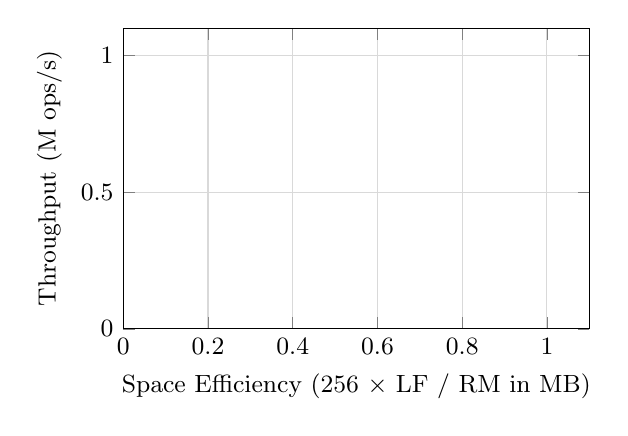
\begin{tikzpicture}
    \begin{axis}[
        width=7.5cm,
        height=5.4cm,
        xlabel={Space Efficiency (256 $\times$ LF / RM in MB)},
        ylabel={Throughput (M ops/s)},
        xmin=0,
        ymin=0,
        grid=major,
        grid style={gray!30},
        legend to name={spaceeff-legend},
        legend entries={Cuckoo, Iceberg, Junction, TPHT, Blast},
        legend cell align=left,
        legend style={draw=none, /tikz/every even column/.style={column sep=0.8em}},
        tick label style={font=\small},
        label style={font=\small},
        scaled ticks=true,
        tick label style={/pgf/number format/fixed,/pgf/number format/precision=2}
    ]
    \AddAllObjectPlotsForCase{1}
    \end{axis}
    \end{tikzpicture}
    \caption{Case 1}
    \end{subfigure}\hfill

    % Case 6
    \begin{subfigure}[b]{0.45\textwidth}
    \centering
    \begin{tikzpicture}
    \begin{axis}[
        width=7.5cm,
        height=5.4cm,
        xlabel={Space Efficiency (256 $\times$ LF / RM in MB)},
        ylabel={Throughput (M ops/s)},
        xmin=0,
        ymin=0,
        grid=major,
        grid style={gray!30},
        tick label style={font=\small},
        label style={font=\small},
        scaled ticks=true,
        tick label style={/pgf/number format/fixed,/pgf/number format/precision=2}
    ]
    % No legend here; legend is separated below
    \addplot[CuckooLineStyle] table[
        x expr=256*\thisrow{load_factor}/\thisrow{avg_real_memory_case1 (MB)},
        y expr=\thisrow{avg_throughput (ops/s)}/1000000,
        restrict expr to domain={\thisrow{object_id}}{6:6},
        restrict expr to domain={\thisrow{case_id}}{6:6}
    ] {\throughputdata};

    \addplot[IcebergLineStyle] table[
        x expr=256*\thisrow{load_factor}/\thisrow{avg_real_memory_case1 (MB)},
        y expr=\thisrow{avg_throughput (ops/s)}/1000000,
        restrict expr to domain={\thisrow{object_id}}{7:7},
        restrict expr to domain={\thisrow{case_id}}{6:6}
    ] {\throughputdata};

    \addplot[JunctionLineStyle] table[
        x expr=256*\thisrow{load_factor}/\thisrow{avg_real_memory_case1 (MB)},
        y expr=\thisrow{avg_throughput (ops/s)}/1000000,
        restrict expr to domain={\thisrow{object_id}}{15:15},
        restrict expr to domain={\thisrow{case_id}}{6:6}
    ] {\throughputdata};

    \addplot[TPHTLineStyle] table[
        x expr=256*\thisrow{load_factor}/\thisrow{avg_real_memory_case1 (MB)},
        y expr=\thisrow{avg_throughput (ops/s)}/1000000,
        restrict expr to domain={\thisrow{object_id}}{17:17},
        restrict expr to domain={\thisrow{case_id}}{6:6}
    ] {\throughputdata};

    \addplot[BlastLineStyle] table[
        x expr=256*\thisrow{load_factor}/\thisrow{avg_real_memory_case1 (MB)},
        y expr=\thisrow{avg_throughput (ops/s)}/1000000,
        restrict expr to domain={\thisrow{object_id}}{20:20},
        restrict expr to domain={\thisrow{case_id}}{6:6}
    ] {\throughputdata};

    \end{axis}
    \end{tikzpicture}
    \caption{Case 6}
    \end{subfigure}

    \vspace{0.6em}

    % Case 7
    \begin{subfigure}[b]{0.45\textwidth}
    \centering
    \begin{tikzpicture}
    \begin{axis}[
        width=7.5cm,
        height=5.4cm,
        xlabel={Space Efficiency (256 $\times$ LF / RM in MB)},
        ylabel={Throughput (M ops/s)},
        xmin=0,
        ymin=0,
        grid=major,
        grid style={gray!30},
        tick label style={font=\small},
        label style={font=\small},
        scaled ticks=true,
        tick label style={/pgf/number format/fixed,/pgf/number format/precision=2}
    ]
    % No legend here; legend is separated below
    \addplot[CuckooLineStyle] table[
        x expr=256*\thisrow{load_factor}/\thisrow{avg_real_memory_case1 (MB)},
        y expr=\thisrow{avg_throughput (ops/s)}/1000000,
        restrict expr to domain={\thisrow{object_id}}{6:6},
        restrict expr to domain={\thisrow{case_id}}{7:7}
    ] {\throughputdata};

    \addplot[IcebergLineStyle] table[
        x expr=256*\thisrow{load_factor}/\thisrow{avg_real_memory_case1 (MB)},
        y expr=\thisrow{avg_throughput (ops/s)}/1000000,
        restrict expr to domain={\thisrow{object_id}}{7:7},
        restrict expr to domain={\thisrow{case_id}}{7:7}
    ] {\throughputdata};

    \addplot[JunctionLineStyle] table[
        x expr=256*\thisrow{load_factor}/\thisrow{avg_real_memory_case1 (MB)},
        y expr=\thisrow{avg_throughput (ops/s)}/1000000,
        restrict expr to domain={\thisrow{object_id}}{15:15},
        restrict expr to domain={\thisrow{case_id}}{7:7}
    ] {\throughputdata};

    \addplot[TPHTLineStyle] table[
        x expr=256*\thisrow{load_factor}/\thisrow{avg_real_memory_case1 (MB)},
        y expr=\thisrow{avg_throughput (ops/s)}/1000000,
        restrict expr to domain={\thisrow{object_id}}{17:17},
        restrict expr to domain={\thisrow{case_id}}{7:7}
    ] {\throughputdata};

    \addplot[BlastLineStyle] table[
        x expr=256*\thisrow{load_factor}/\thisrow{avg_real_memory_case1 (MB)},
        y expr=\thisrow{avg_throughput (ops/s)}/1000000,
        restrict expr to domain={\thisrow{object_id}}{20:20},
        restrict expr to domain={\thisrow{case_id}}{7:7}
    ] {\throughputdata};

    \end{axis}
    \end{tikzpicture}
    \caption{Case 7}
    \end{subfigure}

    % Separated legend below
    \vspace{0.6em}

    {\footnotesize \pgfplotslegendfromname{spaceeff-legend}}

    \caption{Throughput vs Space Efficiency across cases 1, 6, and 7. Space efficiency is 256 $\times$ Load Factor divided by Real Memory (MB), using real memory from case 1 for all cases. Legend shown below for clarity.}
    \label{fig:throughput_space_efficiency_cases}
\end{figure} 

% Include load factor support plots
\section{Load Factor Support Analysis}

\begin{figure}[p]
    \centering
    \begin{tikzpicture}
        \begin{axis}[
            width=12cm,
            height=8cm,
            xlabel={Bin Size},
            ylabel={Load Factor Support (\%)},
            xmode=log,
            xmin=1,
            xmax=200,
            ymin=0,
            ymax=100,
            grid=major,
            grid style={gray!30},
            legend pos=outer north east,
            legend style={font=\small},
            tick label style={font=\small},
            label style={font=\small},
            title={Load Factor Support vs Bin Size},
            title style={font=\small},
            scaled ticks=true,
            tick label style={/pgf/number format/fixed,/pgf/number format/precision=1}
        ]

        % Plot insertion data (from CSV)
        \addplot[CuckooLineStyle] table[
            x=bin_size,
            y index=3,
            col sep=comma,
            restrict expr to domain={\thisrow{object_id}}{4:4}
        ] {\loadfactordata};
        \addlegendentry{Insertion Only}

        % Plot deletion data (hardcoded)
        \addplot[IcebergLineStyle] coordinates {
            (3,7)
            (7,43)
            (15,71)
            (31,85)
            (63,91)
            (127,95)
        };
        \addlegendentry{With Deletion}

        \end{axis}
    \end{tikzpicture}
    \caption{Load Factor Support vs Bin Size for different hash table implementations. The x-axis shows bin size on a logarithmic scale, while the y-axis shows the maximum supported load factor as a percentage.}
    \label{fig:load_factor_support}
\end{figure} 

% Include scaling plots
\section{Scaling Analysis}

% Function to map case numbers to descriptive names
\newcommand{\getCaseName}[1]{%
    \ifnum#1=1 Insertion\fi%
    \ifnum#1=3 Deletion\fi%
    \ifnum#1=6 Positive Query\fi%
    \ifnum#1=7 Negative Query\fi%
}

% Helper macro to plot all objects for a given case
\newcommand{\AddAllObjectPlotsForScaling}[1]{%
    % Cuckoo (object_id=6)
    \addplot[CuckooLineStyle] table[
        x=thread_num,
        y expr=\thisrow{throughput (ops/s)}/1000000,
        restrict expr to domain={\thisrow{case_id}}{#1:#1},
        restrict expr to domain={\thisrow{object_id}}{6:6}
    ] {\scalingdata};
    
    % Iceberg (object_id=7)
    \addplot[IcebergLineStyle] table[
        x=thread_num,
        y expr=\thisrow{throughput (ops/s)}/1000000,
        restrict expr to domain={\thisrow{case_id}}{#1:#1},
        restrict expr to domain={\thisrow{object_id}}{7:7}
    ] {\scalingdata};
    
    % Junction (object_id=15)
    \addplot[JunctionLineStyle] table[
        x=thread_num,
        y expr=\thisrow{throughput (ops/s)}/1000000,
        restrict expr to domain={\thisrow{case_id}}{#1:#1},
        restrict expr to domain={\thisrow{object_id}}{15:15}
    ] {\scalingdata};
    
    % TPHT (object_id=17)
    \addplot[TPHTLineStyle] table[
        x=thread_num,
        y expr=\thisrow{throughput (ops/s)}/1000000,
        restrict expr to domain={\thisrow{case_id}}{#1:#1},
        restrict expr to domain={\thisrow{object_id}}{17:17}
    ] {\scalingdata};
    
    % Blast (object_id=20)
    \addplot[BlastLineStyle] table[
        x=thread_num,
        y expr=\thisrow{throughput (ops/s)}/1000000,
        restrict expr to domain={\thisrow{case_id}}{#1:#1},
        restrict expr to domain={\thisrow{object_id}}{20:20}
    ] {\scalingdata};
}

% Shared legend above all graphs
\begin{figure}[p]
    \centering
    \begin{tikzpicture}
        \begin{axis}[
                width=12cm,
                height=2cm,
                hide axis,
                legend entries={Cuckoo, Iceberg, Junction, TPHT, Blast},
                legend columns=5,
                legend style={font=\small, column sep=15pt, /tikz/every even column/.append style={column sep=15pt}},
                legend to name={scaling-legend}
            ]
            \addplot[CuckooLineStyle] coordinates {(0,0)};
            \addplot[IcebergLineStyle] coordinates {(0,0)};
            \addplot[JunctionLineStyle] coordinates {(0,0)};
            \addplot[TPHTLineStyle] coordinates {(0,0)};
            \addplot[BlastLineStyle] coordinates {(0,0)};
        \end{axis}
    \end{tikzpicture}
    \vspace{0.5cm}
\end{figure}

\begin{figure}[p]
    \centering
    
    % Display shared legend
    {\footnotesize \pgfplotslegendfromname{scaling-legend}}
    \vspace{0.3cm}

    % Case 1
    \begin{subfigure}[b]{0.48\textwidth}
        \centering
        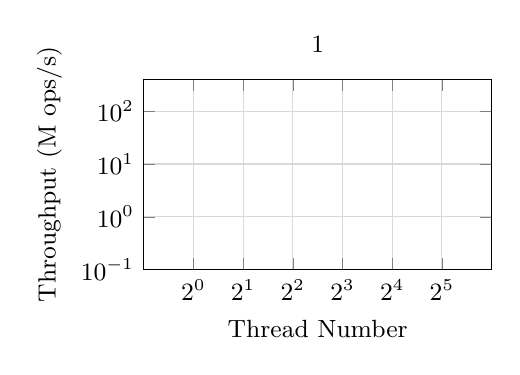
\begin{tikzpicture}
            \begin{axis}[
                    width=6cm,
                    height=4cm,
                    xlabel={Thread Number},
                    ylabel={Throughput (M ops/s)},
                    xmode=log,
                    ymode=log,
                    log basis x=2,
                    log basis y=10,
                    xmin=0.5,
                    xmax=64,
                    ymin=0.1,
                    ymax=400,
                    xtick={1,2,4,8,16,32},
                    ytick={0.1,1,10,100},
                    grid=major,
                    grid style={gray!30},
                    tick label style={font=\small},
                    label style={font=\small},
                    title={\getCaseName{1}},
                    title style={font=\small},
                    scaled ticks=true,
                    tick label style={/pgf/number format/fixed,/pgf/number format/precision=1}
                ]

                \AddAllObjectPlotsForScaling{1}

            \end{axis}
        \end{tikzpicture}
        \caption{\getCaseName{1}}
    \end{subfigure}
    \hfill
    % Case 3
    \begin{subfigure}[b]{0.48\textwidth}
        \centering
        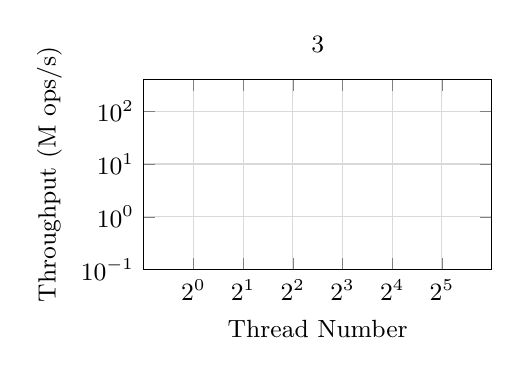
\begin{tikzpicture}
            \begin{axis}[
                    width=6cm,
                    height=4cm,
                    xlabel={Thread Number},
                    ylabel={Throughput (M ops/s)},
                    xmode=log,
                    ymode=log,
                    log basis x=2,
                    log basis y=10,
                    xmin=0.5,
                    xmax=64,
                    ymin=0.1,
                    ymax=400,
                    xtick={1,2,4,8,16,32},
                    ytick={0.1,1,10,100},
                    grid=major,
                    grid style={gray!30},
                    tick label style={font=\small},
                    label style={font=\small},
                    title={\getCaseName{3}},
                    title style={font=\small},
                    scaled ticks=true,
                    tick label style={/pgf/number format/fixed,/pgf/number format/precision=1}
                ]

                \AddAllObjectPlotsForScaling{3}

            \end{axis}
        \end{tikzpicture}
        \caption{\getCaseName{3}}
    \end{subfigure}

    % Case 6
    \begin{subfigure}[b]{0.48\textwidth}
        \centering
        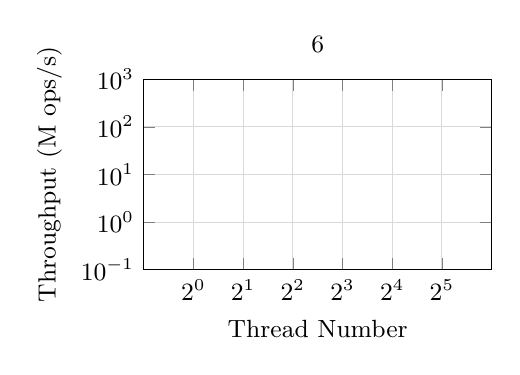
\begin{tikzpicture}
            \begin{axis}[
                    width=6cm,
                    height=4cm,
                    xlabel={Thread Number},
                    ylabel={Throughput (M ops/s)},
                    xmode=log,
                    ymode=log,
                    log basis x=2,
                    log basis y=10,
                    xmin=0.5,
                    xmax=64,
                    ymin=0.1,
                    ymax=1000,
                    xtick={1,2,4,8,16,32},
                    ytick={0.1,1,10,100,1000},
                    grid=major,
                    grid style={gray!30},
                    tick label style={font=\small},
                    label style={font=\small},
                    title={\getCaseName{6}},
                    title style={font=\small},
                    scaled ticks=true,
                    tick label style={/pgf/number format/fixed,/pgf/number format/precision=1}
                ]

                \AddAllObjectPlotsForScaling{6}

            \end{axis}
        \end{tikzpicture}
        \caption{\getCaseName{6}}
    \end{subfigure}
    \hfill
    % Case 7
    \begin{subfigure}[b]{0.48\textwidth}
        \centering
        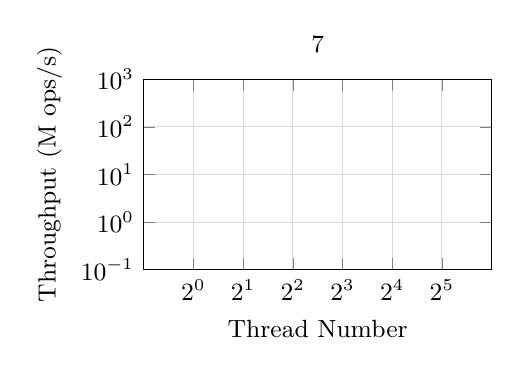
\begin{tikzpicture}
            \begin{axis}[
                    width=6cm,
                    height=4cm,
                    xlabel={Thread Number},
                    ylabel={Throughput (M ops/s)},
                    xmode=log,
                    ymode=log,
                    log basis x=2,
                    log basis y=10,
                    xmin=0.5,
                    xmax=64,
                    ymin=0.1,
                    ymax=1000,
                    xtick={1,2,4,8,16,32},
                    ytick={0.1,1,10,100,1000},
                    grid=major,
                    grid style={gray!30},
                    tick label style={font=\small},
                    label style={font=\small},
                    title={\getCaseName{7}},
                    title style={font=\small},
                    scaled ticks=true,
                    tick label style={/pgf/number format/fixed,/pgf/number format/precision=1}
                ]

                \AddAllObjectPlotsForScaling{7}

            \end{axis}
        \end{tikzpicture}
        \caption{\getCaseName{7}}
    \end{subfigure}

    \caption{Scaling Analysis for different hash table implementations across various operations. Each subfigure shows throughput scaling with thread count for a specific operation type.}
    \label{fig:scaling_analysis}
\end{figure}

% Include percentile tables
\begin{table}[h!]
    \centering
    \tiny
    \caption{Latency Percentiles for Insertion Operations}
    \label{tab:latency_percentiles_insertion}
    \begin{tabular}{|c|ccccc|}
        \toprule
        Percentile & Cuckoo & Iceberg & Junction & TPHT & Blast \\
        \midrule
        $50.0\%$ & 202 & 226 & 436 & 367 & 195 \\
        $95.0\%$ & 914 & 555 & 36971 & 631 & 468 \\
        $99.0\%$ & 2333 & 856 & 66098 & 812 & 608 \\
        $99.9\%$ & 6270 & 13950 & 112224 & 1080 & 874 \\
        $99.99\%$ & 124908 & 17488 & 293696 & 3630 & 3033 \\
        max & 800721058 & 141461798 & 42000209 & 77782769 & 178965795 \\
        \bottomrule
    \end{tabular}
\end{table}

\begin{table}[h!]
    \centering
    \tiny
    \caption{Latency Percentiles for Positive Query Operations}
    \label{tab:latency_percentiles_positive_query}
    \begin{tabular}{|c|ccccc|}
        \toprule
        Percentile & Cuckoo & Iceberg & Junction & TPHT & Blast \\
        \midrule
        $50.0\%$ & 114 & 231 & 152 & 283 & 189 \\
        $95.0\%$ & 158 & 488 & 718 & 556 & 322 \\
        $99.0\%$ & 187 & 648 & 1347 & 724 & 546 \\
        $99.9\%$ & 431 & 892 & 2307 & 991 & 655 \\
        $99.99\%$ & 125414 & 3508 & 3259 & 3446 & 1183 \\
        max & 800572948 & 84186 & 84616 & 211481 & 76530 \\
        \bottomrule
    \end{tabular}
\end{table}

\begin{table}[h!]
    \centering
    \tiny
    \caption{Latency Percentiles for Negative Query Operations}
    \label{tab:latency_percentiles_negative_query}
    \begin{tabular}{|c|ccccc|}
        \toprule
        Percentile & Cuckoo & Iceberg & Junction & TPHT & Blast \\
        \midrule
        $50.0\%$ & 107 & 174 & 153 & 137 & 125 \\
        $95.0\%$ & 132 & 473 & 727 & 339 & 172 \\
        $99.0\%$ & 173 & 652 & 1363 & 551 & 398 \\
        $99.9\%$ & 373 & 1042 & 2327 & 783 & 565 \\
        $99.99\%$ & 125436 & 2046 & 3281 & 1113 & 675 \\
        max & 819076828 & 45610 & 290174 & 38802 & 34051 \\
        \bottomrule
    \end{tabular}
\end{table}

\end{document}
